\documentclass[11pt,oneside]{article}
\usepackage[letterpaper,margin=1in]{geometry}
\usepackage{booktabs,tabularx,array,graphicx,amsmath,amssymb,xcolor}
\usepackage{float}
\usepackage[numbers]{natbib}
\usepackage[colorlinks=true,urlcolor=blue,citecolor=blue]{hyperref}
\usepackage{enumitem}
\setlength{\parindent}{0pt}
\setlength{\parskip}{4pt}
\setlength{\emergencystretch}{2em}
\renewcommand{\arraystretch}{1.08}
\title{CS781 Capstone Project:\\In-House Legal Intelligence System}
\author{Krishna KKarthikeya G N\\Roll number 250564\\Indian Institute of Technology Kanpur}
\date{9 November 2026 -- evidence freeze}
\begin{document}
\maketitle
\begin{abstract}
This report traces seven legal NLP tasks from an in-house language model to retrieval. A 12-layer, width-768 causal model with a learned 32,768-token byte-BPE vocabulary and prompt-aware copy route was trained from scratch on the permitted legal sources. Its descendants and other in-house checkpoints supported exact-span NER, judgment prediction, statute identification, and summarization; prediction-level combinations were evaluated separately from neural backbones. The highest recorded Codabench submissions score 0.8341, 0.5130, 0.6723, 0.3949, 0.7847, and 0.4064 in Phases 1, 2, 4, 5, 6, and 7 respectively. Phase 3 has prepared code but no recorded scored submission. The comparisons expose the value of exact output contracts, sparse lexical evidence, calibrated combinations, and the limits of short held-out splits. Local and hidden scores are reported separately.
\end{abstract}

\section{Competition Result}
The account shown on Codabench is \texttt{k\_250564}; the roll number is 250564. Table~\ref{tab:official} records the highest \emph{finished and scored} submission visible on 9 November 2026. A dash means the evidence does not establish the requested value, rather than a zero score. The live leaderboard showed Phase 1 rank 49; ranks for other phases were not captured reliably at this freeze.
\begin{table}[h]
\centering\small
\caption{Official Codabench results, frozen 9 November 2026. ``Rows'' counts displayed submission records, including duplicate, failed, and pending records; it is not the number of distinct valid submissions.}
\label{tab:official}
\begin{tabular}{clccc}
\toprule Phase & Task & Best primary score & Rank & Rows \\\midrule
1 & Legal LM continuation & 0.8341 BERTScore F1 & 49 & 17 \\
2 & Exact-span NER & 0.5130 macro-F1 & -- & 16 \\
3 & Rhetorical roles & no scored submission & -- & 0 \\
4 & Judgment prediction & 0.6723 macro-F1 & -- & 16 \\
5 & Statute identification & 0.3949 macro-F1 & -- & 9 \\
6 & Abstractive summarization & 0.7847 BERTScore F1 & -- & 15 \\
7 & Prior case retrieval & 0.4064 micro-F1@7 & -- & 23 \\
\bottomrule
\end{tabular}
\end{table}
The displayed records total 96, but that includes repeated uploads and unscored failures; the number of \emph{distinct valid} submissions cannot be inferred from it. Phase 3 did not meet the four-distinct-submission requirement. The other phases have at least four visibly different finished filenames, except Phase 5 where the visible filenames likewise exceed four; this is a filename-level check, not an organizer eligibility ruling. Phase 3 is a material missing deliverable.

\section{Introduction and Problem Description}
The project asks whether legal text processing can be built around an in-house model and the course's own data, within restricted compute and a 50--300 million parameter Phase 1 bound. The phases are connected in motivation, but their metrics are not interchangeable. Phase 1 continues a 512-word prompt by 128 words and is evaluated mainly by BERTScore F1 \cite{zhang2020bertscore}; Phase 2 returns exact character-span triples for 12 entity classes and uses macro-F1; Phase 3 labels the supplied sentences with rhetorical roles; Phase 4 predicts a binary judgment outcome; Phase 5 selects multiple statute IDs and is scored by macro-F1 on the live task page; Phase 6 produces an abstractive summary scored by BERTScore F1; Phase 7 ranks seven prior-case IDs per query and uses micro-F1@7. The supplied template says Micro-F1 for Phase 5 in a Results prompt, whereas its current Codabench page calls Macro-F1 the primary metric. We use the live page's designation and retain micro-F1 as a secondary local measure.

The research path moved from language-model continuation to task adaptation, then to long-document aggregation and probability fusion. The comparisons ask which improvements survive the hidden evaluation, and which arise from exploiting a small development split. External pretrained legal language models and outside legal corpora were outside the Phase 1 foundation constraint. The report covers completed and evidenced runs; it does not call prepared Phase 3 notebooks a completed experiment, or a reconstructed notebook an original executed run.

\section{Data Analysis and Preprocessing}
\subsection{Sources and official splits}
Phase 1 used the four permitted text families: Acts, High Court judgments, Supreme Court judgments, and Tribunal decisions. The archived tokenizer and training streams are source linked, but a trustworthy four-source token-count table was not recovered for this report, so no mixing-ratio effect is claimed. The official Phase 4 binary train set contains 32,305 cases, the dev set 994, and the held-out test set 1,517. Phase 5's saved run records identify 38,113 fitting examples, 4,313 training-calibration examples, 10,181 dev cases, and 13,019 test cases. Phase 7's archived local evaluation has 118 labeled dev queries and 237 test queries. These denominators matter: comparing a 16-example summarization probe with an official hidden score would invite a false conclusion.

\subsection{Corpus statistics that actually informed design}
Table~\ref{tab:data} is recomputed directly from the preserved Phase 4 JSON, using whitespace word counts. Training labels are 18,920 zeros and 13,385 ones; the official dev split is exactly balanced, 497/497. The longest training case has 412,606 whitespace tokens. A fixed 512-token prefix therefore discards most text in many cases. This observation motivates the recorded ordered-window policy, including tail windows, but does not itself prove that the decision always appears near the end.
\begin{table}[h]
\centering\small
\caption{Our Phase 4 data audit (whitespace words, not model BPE tokens).}
\label{tab:data}
\begin{tabular}{lrrrrr}\toprule Split & Cases & Class 0 & Class 1 & Median words & 90th percentile \\\midrule
Train & 32,305 & 18,920 & 13,385 & 2,035 & 6,449 \\
Dev & 994 & 497 & 497 & 2,822 & 6,897 \\
\bottomrule\end{tabular}
\end{table}
The Phase 5 LoRA evaluation record contains 100 labels. On 10,181 dev cases, support ranges from 68 to 2,936 per label (median 175), and three labels have zero F1. This measured imbalance explains why micro- and macro-F1 diverge: frequent labels can dominate the micro aggregate while each rare label still contributes equally to macro-F1. Exact class names and comparable class-wise tables for Phases 2 and 3 were not recovered; we do not invent them.
\begin{table}[h]
\centering\small
\caption{Our audit of Phase 5 saved evaluation metadata; support and zero-F1 counts come from the LoRA dev report, while split sizes come from the sparse-hybrid report.}
\label{tab:phase5data}
\begin{tabular}{lr@{\qquad}lr}\toprule Quantity & Value & Quantity & Value \\\midrule
Fitting cases & 38,113 & Calibration cases & 4,313 \\
Dev cases & 10,181 & Test cases & 13,019 \\
Distinct labels & 100 & Median label support & 175 \\
Minimum label support & 68 & Maximum label support & 2,936 \\
LoRA labels with zero dev F1 & 3 & & \\
\bottomrule\end{tabular}
\end{table}

\subsection{Preprocessing}
The Phase 1 learner trains byte BPE from the approved corpus \cite{sennrich2016bpe}; byte fallback retains citations, section signs, names, and punctuation without an unknown-token bucket. The Phase 2 code maps original character positions through tokenized windows, then reconstructs BIO spans on the \emph{unmodified source string}. Its first-four runner uses 1,600-character windows with 240-character overlap and at most 768 tokens per window. Normalizing whitespace or lowercasing before recovering offsets would change exact boundaries and lose strict-span credit. Phase 3's saved notebooks are prepared but have no verified executed sentence-level output to analyze. Phase 4 preserves ordered 512-token windows, up to 16 unique windows, including the document tail; the long-tail audit above explains the need for that design. Phase 5 joins sparse full-document features with a B1 neural branch, so its lexical route can still see statute names after neural truncation. Phase 7 uses the official candidate pool and must exclude a query's own ID from its seven predictions; the later corrected exports implement that contract.

\section{Approach and Model Evolution}
\subsection{Phase-1 foundation model}
The winning LegalSpan run extends a 12-block, 768-wide causal Transformer \cite{vaswani2017attention}, with 12 heads, a 2,048-wide feed-forward branch, rotary positions, RMSNorm, and SwiGLU. The submitted config specifies a 32,768-token own byte-BPE vocabulary, an 8,192-token maximum sequence, a 128-wide prompt route in the upper four blocks, and gradient checkpointing. The route attends to eligible prompt positions with role and continuity cues; a learned gate blends this route into the residual stream. At generation, a second gate blends vocabulary probabilities with copying from prompt tokens. Causality requires every route key used at generation step $t$ to come from visible prompt positions or prior tokens, never future target positions. The archived run metadata records \textbf{112,095,887 unique parameters}, inside the course's 50--300 million bound, and its training code checks the same bound before a non-smoke run.

The common objective is next-token negative log likelihood, $-\sum_t\log p_\theta(x_t\mid x_{<t})$. The copy/generation mixture is related to pointer-generator work \cite{see2017pointer}, although this implementation's prompt route is its own recorded variant. Training starts from random model weights on the approved sources; the BERTScore evaluator's encoder was not used to initialize the participant model. The archive config sets learning rate $3\times10^{-4}$, gradient accumulation 32, a target of 209.9 million target tokens, and a 1 million-token pilot. The completed status records \textbf{11,888 optimizer steps and 209,927,459 target tokens} in 21,988 seconds; Figure~\ref{fig:p1curve} uses the original loss log. Selection compared model checkpoints and decoding policies for a 128-word continuation. The denser A run achieved 0.8304, whereas LegalSpan reached 0.8341 on Codabench. The 0.0037 difference is consistent with a useful copy route, but distinct checkpoints and decode settings prevent isolating that mechanism causally.

\subsection{Transfer protocol (Phases 2--7)}
The project did not train one universal seven-head network. It preserved several Phase 1 lineages and fine-tuned or adapted separate descendants; some final predictions then combine independent models. Full tuning, frozen-backbone low-rank updates, LoRMA, adapter-like modules, distillation, and prediction-level stacking appear in the source histories. The course constraint is met at the individual backbone level; an ensemble is explicitly labeled as a different prediction procedure. It would be inaccurate to attribute a stack's hidden score to one B1 architecture.

\subsection{Phase 2 - Legal NER}
The final two-of-four consensus is a rule over predictions, not an extra trained model. Its four input encoders (LegalSpan, B1, C1, A0) produce BIO token/character features; the first-four runner combines token context, a 32-dimensional character embedding, and a 128-unit bidirectional GRU before constrained BIO decoding. A candidate survives when at least two models agree on the exact $(\mathrm{start},\mathrm{end},\mathrm{label})$ triple; conflicting overlaps are ranked by vote and length. This targets spurious boundaries, where an almost-correct entity is still a strict failure. The local 12-document strict macro-F1 is 0.4631 and the finished Codabench score 0.5130. The local gain mechanism is plausible, but a small held-out set cannot establish its reliability across all 12 types.

\subsection{Phase 3 - Rhetorical role prediction}
The local folder contains four adaptation notebooks for sentence-level rhetorical-role experiments, following D222 LoRMA, B1 LoRA, C1 IA3, and A0 distillation paths. No completed metrics or Codabench submission were found. The intended question was whether neighboring sentence context helps distinguish roles across Corporate Law and IT text; there is no evidence here to resolve it. Consequently this phase is documented as prepared code, not a trained or best-performing system.

\subsection{Phase 4 - Court judgment prediction}
Earlier baselines included a full-data B1 reference (0.6145 hidden), a GRU-only document head (0.6223), and a Transformer-only head continued to v7 (0.6641). The winning prediction procedure takes probabilities from v7 Transformer, v6 Transformer, v5 GRU, and v4 reference. A regularized logistic combiner is fit on 512 training-calibration cases, with coefficients $(0.5568,0.3330,0.3002,0.3513)$ and intercept $-0.0340$: $q=\sigma(b+\sum_{i=1}^{4}w_ip_i)$; output is one when $q\geq0.5$. Five-fold calibration CV is 0.7107 macro-F1, exploratory official dev is 0.6940 on 994 cases, and Codabench is 0.6723. Because the dev set helped compare several stack families, the dev estimate is post-selection and may be optimistic. The hidden score is the relevant independent comparison.

\subsection{Phase 5 - Legal statute identification}
The winning sparse hybrid blends a B1 LoRA branch with a full-document sparse classifier. Training-only grouped calibration chose a sparse weight of 0.9 and per-label thresholds; each label receives its own sigmoid score before thresholding. This keeps exact statute names and citations visible even when the neural route sees only a subset of a long case. The source report gives local dev macro-F1 0.3909 and micro-F1 0.5000; Codabench macro-F1 is 0.3949. The small neural weight does not show that neural context is useless: it shows that, for this label distribution and calibration, sparse evidence carried most of the predictive mass. A separate CV-tuned hybrid scored 0.3944 on Codabench, showing that a slightly higher local score did not transfer.

\subsection{Phase 6 - Abstractive summarization}
The best scored model adapts the own LegalSpan causal decoder with low-rank updates \cite{hu2022lora} and retains its prompt-aware route/copy behavior. The alternative families include B1 fusion and length control, B1 AdaLoRA, C1 Houlsby adapters, D222 prefix tuning, and A0 sequence-level distillation. Long judgments are packed or compressed before generation; generation length and repetition controls matter because BERTScore can reward fluent overlap without guaranteeing correct legal holdings. LegalSpan LoRA achieved 0.7847 hidden BERTScore F1. A local 16-example HIF probe reached 0.8358, but it was not a hidden submission and is too small to supersede the official result.

\subsection{Phase 7 - Prior Case Retrieval (PCR)}
The retrieval experiments mix a lexical similarity route with learned dense scores from full, partial, LoRMA, and distilled variants. Scores are combined to rank candidates, then seven unique in-pool IDs are emitted per query. A corrected export removed self-matches; the selected ensemble and full-model export tie at 0.4064 hidden micro-F1@7. The earlier local ensemble result of 0.4158 on 118 queries predates the correction, so it cannot be presented as the corrected model's dev score. A lexical-only corrected submission scored 0.4022; the small hidden difference suggests the dense branch provided some complementary ranking information, but does not isolate which queries benefited.

\section{Experiments and Implementation Details}
\subsection{Compute and training protocol}
The preserved lineages contain local and Kaggle/Colab-style runs, checkpoints, source hashes, and exported prediction ZIPs. The Phase 4 head-ablation continuation used two T4 GPUs, one worker per GPU; its v7 manifest verifies exact resume from v6 optimizer states and checkpoint saves. The common Phase 2 first-four runner used AdamW, cosine warmup/decay, eight-window accumulation, and checkpoint selection by strict held-out macro-F1. Phase 1 LegalSpan's saved config specifies the optimizer settings above, gradient clipping, and periodic checkpoints. Phase 5 reports choose thresholds on a training-calibration split rather than official dev. Phase 6 variants use distinct adaptation schedules; a single hyperparameter row for all of them would be misleading. Full run-specific configs remain with the code. We do not infer an epoch count from an exported ZIP or call a time-budget pause convergence.

\subsection{Local evaluation}
Local sets served different purposes: Phase 2 used a 12-document holdout from 70 labeled documents; Phase 4 used 512 training-calibration cases and separately 994 official dev cases; Phase 5 used 4,313 calibration and 10,181 dev cases; Phase 7's saved pre-correction evaluation used 118 queries. These are not the Codabench hidden sets. The Phase 4 stack's 0.7107 calibration CV versus 0.6723 hidden difference (0.0384) is a concrete warning against treating a small tuning split as the final score. Local Phase 5 macro-F1 0.3909 and hidden 0.3949 happen to be close; that agreement should not be generalized to other variants.

\subsection{Ablations and controlled comparisons}
Table~\ref{tab:ablate} separates informative comparisons from claims they cannot prove. A strict causal ablation would hold training data, checkpoint lineage, decode settings, and compute constant while changing one factor. Several historical submissions change more than one of these, so their score differences support prioritization rather than a proof about a component.
\begin{table}[H]\centering\small
\caption{Measured comparisons and inference limits; all values in the right column are official hidden primary metrics.}
\label{tab:ablate}
\begin{tabularx}{\linewidth}{lXr}\toprule Phase & Variant & Score \\\midrule
1 & Dense A; LegalSpan; B0 encoder--decoder & 0.8304; 0.8341; 0.7972 \\
2 & C1 full; B1 LoRA; D222 continued; 2-of-4 vote & 0.3779; 0.4406; 0.5067; 0.5130 \\
4 & B1 reference; GRU-only; Transformer v7; four-model stack & 0.6145; 0.6223; 0.6641; 0.6723 \\
5 & B1 LoRA; sparse-guided; sparse hybrid & 0.2554; 0.2417; 0.3949 \\
6 & B1 AdaLoRA; B1 length; LegalSpan LoRA & 0.7656; 0.7783; 0.7847 \\
7 & Lexical corrected; KD corrected; ensemble corrected & 0.4022; 0.4034; 0.4064 \\
\bottomrule\end{tabularx}
\end{table}

\section{Results}
The best visible submissions are in Table~\ref{tab:official}; Table~\ref{tab:ablate} gives at least three distinct methods for each completed phase. Phase 3 has no score and therefore no honest variant ranking. The Phase 1 LegalSpan gain over A is 0.0037 BERTScore F1, while the Phase 2 exact-span vote exceeds the strongest displayed individual D222 continued run by 0.0063 macro-F1. Phase 4's stack exceeds the strongest constituent submitted separately, v7 Transformer, by 0.0082 macro-F1. Phase 5's sparse hybrid exceeds the B1 LoRA submission by 0.1395 macro-F1; this larger gap is compatible with the long-document lexical coverage hypothesis, though the systems also differ in calibration and training. Phase 6 LegalSpan LoRA exceeds the B1 fusion length candidate by 0.0064 BERTScore F1. Phase 7's corrected ensemble exceeds corrected lexical fallback by 0.0042 micro-F1@7.

Figure~\ref{fig:p1curve} plots the original LegalSpan training NLL against realized target tokens. Its median drops from 2.96 across the first 50 logged points to 1.08 across the last 50. This is training improvement, not a held-out perplexity curve or direct evidence of better generation. Figure~\ref{fig:p5curve} plots measured training-calibration macro-F1 after each epoch for three Phase 5 neural candidates. All three rise across four recorded epochs; sparse-guided rises from 0.2053 to 0.2466. This does not prove that further epochs would improve hidden performance. Class-wise Phase 2/3 scores were not recovered. For Phase 7, the pre-correction local lexical baseline had 357 true positives, 469 false positives and 616 false negatives over 118 dev queries (micro-F1 0.3969); its selected ensemble had 0.4158 before the self-match correction. That local comparison is not the same as the corrected hidden comparison above.
\begin{figure}[ht]
\centering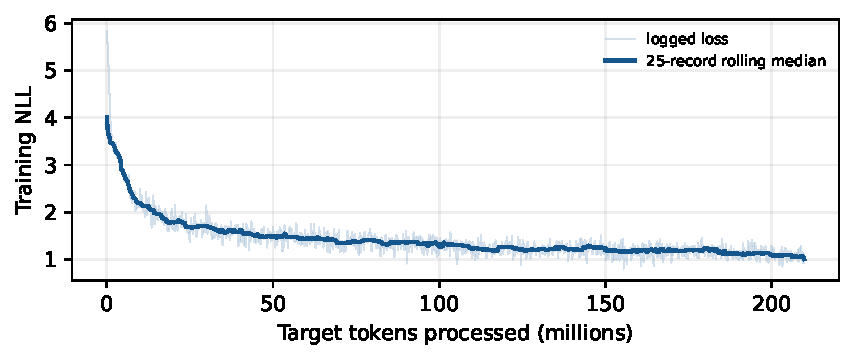
\includegraphics[width=0.72\linewidth]{figure_phase1_training_loss.pdf}
\caption{Phase 1 LegalSpan training loss from 1,189 archived log records. The dark line is a 25-record rolling median; no validation loss is implied.}
\label{fig:p1curve}
\end{figure}
\begin{figure}[ht]
\centering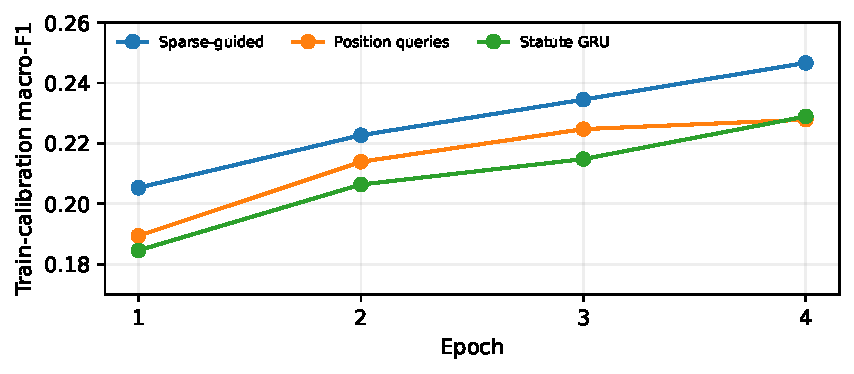
\includegraphics[width=0.72\linewidth]{figure_phase5_calibration.pdf}
\caption{Phase 5 calibration learning curves from archived epoch histories. This is training-derived calibration, not official dev or hidden test.}
\label{fig:p5curve}
\end{figure}

\section{Error Analysis and Discussion}
\subsection{Phase-wise failure modes}
In Phase 1, a fluent continuation can miss the cited section or party even if BERTScore is high; the copy route addresses that specific failure but can also copy irrelevant material. In Phase 2, a one-character boundary shift makes an otherwise right entity an exact-span false positive plus false negative. The voting procedure preferentially removes singleton spans, increasing precision at potential recall cost; the local consensus record reports macro precision 0.5079 and recall 0.4419, consistent with that trade-off. Phase 3 cannot be error-analyzed empirically without completed predictions. Phase 4's train/dev balance shift and long cases create two observable hazards: threshold sensitivity and losing outcome text under prefix-only truncation. Phase 5's three zero-F1 labels in the LoRA local report identify a rare-label failure mode; sparse features help when explicit statute identifiers appear but may miss paraphrases. Phase 6 BERTScore does not verify whether a generated legal proposition is true. Phase 7's self-match correction was essential because an apparently strong ranking that includes the query itself violates the output contract.

\subsection{What the metrics do not measure}
ROUGE \cite{lin2004rouge}, BLEU \cite{papineni2002bleu}, and BERTScore measure overlap or semantic similarity to references, not legal correctness. Exact-span F1 punishes even slight offset disagreement, while a judge may regard the reference and predicted phrase as equivalent. Retrieval F1@7 does not tell a lawyer why a case is relevant. A firm deployment would require citation verification, factual review, and traceable source passages, beyond these leaderboard scores.

\subsection{Limitations and what you would do next}
The decisive limitation is the missing scored Phase 3 work. Other limitations are small local holdouts, post-selection comparison on official dev, unavailable source-wise token counts, missing per-class NER and rhetorical-role breakdowns, and incomplete live rank capture. The next controlled Phase 4 experiment would hold the same B1 checkpoint and training budget fixed while changing only head aggregation. For Phase 5, compare sparse-only and hybrid scores per rare label and citation pattern. For Phase 7, recompute the corrected ensemble on the fixed 118-query dev manifest before claiming any local gain. None of these proposed tests is reported as performed.

\subsection{Surprising findings}
The large Phase 5 advantage of a 90\% sparse mixture over a B1 LoRA-only submission was not what a purely neural-transfer story would predict. It is understandable given long documents and explicit statute references, but the hidden score alone cannot establish the full causal explanation. Also, the Phase 4 six-model stack underperformed the simpler four-model stack on the hidden test (0.6677 versus 0.6723), despite additional model inputs. More models did not guarantee better generalization.

\section{Conclusion}
The verified results support three practical lessons. First, preserve exact output contracts: character offsets and self-exclusion can dominate a seemingly sophisticated architecture. Second, preserve relevant evidence across long documents: ordered windows, lexical statute features, and query-aware copy routes each address a specific truncation or grounding risk. Third, treat ensembling and tuning estimates cautiously; Phase 4's four-model stack improved the hidden score, but its calibration CV was materially higher. The project has several strong scored phases and a documented gap in Phase 3. Its final scientific claim is the observed sequence of experiments and scores, not a proof that any single component is universally best.

\clearpage
\section*{LLM Usage Declaration}
\textbf{Q1. Models and vendor.} OpenAI ChatGPT/Codex was used during planning, implementation support, analysis drafting, and assembly of this report. The exact model version for every earlier chat is not recoverable from the preserved artifacts and should not be guessed.

\textbf{Q2. Scope of use.} The following is an explicit disclosure of the work represented in this report. ``Yes'' includes work for which the assistant generated drafts or substantial code, even if the student prompted, reviewed, or revised it. A claim that AI was only a grammar checker or an ancillary debugger would be inaccurate for these materials.
\begin{table}[H]\centering\small
\begin{tabularx}{\linewidth}{p{4.5cm}cX}\toprule Activity & LLM? & Specific use \\\midrule
Understanding concepts and papers & Yes & Explained attention, BPE, low-rank adaptation, copying, metrics and constraints; source papers still require direct reading. \\
High-level brainstorming & Yes & Compared candidate architectures, long-context policies, transfer options, sparse features and ensembles. \\
Model design and mathematics & Yes & Helped formalize routes, gating, tensor shapes, losses and possible limitations; design authorship must be described accurately. \\
Core code and integration & Yes & Generated or modified training/inference modules in some lineages; helped connect token IDs, masks, offsets, projections, checkpoint states and output schemas. \\
Ancillary debugging and plots & Yes & Assisted with checkpoint/resume logic, tensor dimensions, export validation, hashing and visualization scripts. \\
Hyperparameter or threshold search & Yes & Assisted with search scripts and reasoning around calibration; measured selection used the saved runs and data partitions. \\
Results analysis and conclusions & Yes & Drafted and edited interpretations, caveats and this report's analysis/conclusion from inspected evidence. \\
Report structure and prose & Yes & Produced a substantial report draft in the supplied section order, edited wording, tables and citations. \\
\bottomrule\end{tabularx}
\end{table}
In particular, the assistant explained the subword-vocabulary trade-off in BPE \cite{sennrich2016bpe}, causal self-attention \cite{vaswani2017attention}, source copying \cite{see2017pointer}, and low-rank updates \cite{hu2022lora}. It helped formalize the LegalSpan route's eligibility mask and copy mixture, check attention and residual tensor dimensions, connect the Phase 2 character map to exact offsets, reason about Phase 4 chunk masks and calibration leakage, and validate that Phase 7 returns seven unique non-self candidate IDs. It also generated code or edits for checkpoint save/resume, optimizer and RNG restoration, run manifests, ZIP contracts and SHA checks. Those are substantive implementation and reasoning contributions, not merely spelling fixes. The exact earlier prompt-by-prompt division of work was not fully recoverable, so this declaration errs toward disclosure.

The screenshots and run artifacts are the source of numeric results. The assistant did not create the historical Codabench scores. The student must check each claim, paper citation, code path and interpretation before submitting; the course's written template restricts some of the uses disclosed above, while the student reports later oral clarification from the instructor. This declaration records actual use rather than assuming the clarification waives disclosure.

\textbf{Q3. Other sources.} The course capstone brief and submission template; official task data and evaluation rules; the original code, checkpoints, logs and prediction receipts; the Codabench account's submission pages; and the papers cited below. Source-level notes in the repository identify additional ideas examined for the LegalSpan route.

\textbf{Q4. Student's own contribution (8--12 sentences).} \emph{To be written by the student, as requested. State the student's own architecture decisions, code work, experiments, interpretation, and at least two failed trials. This must not be filled by the assistant or left blank in a submitted version.}

\bibliographystyle{ieeetr}
\bibliography{references}
\end{document}
